% !TEX root =  root.tex

\section{RESULTS}\label{sec:results}
In figure (\ref{fig:speedup}) the speedups of the matrix inversion algorithm by LU decomposition for various of GPU models are displayed. The speedup is archived against a sequential version of the algorithm running on area-equivalent CPUs, i.e. the Tesla K10 is compared to a Intel Xeon server CPU, the GT 730 is compared to a desktop CPU and the GT 525M to a Intel i5 mobile CPU. 
\begin{figure*}
	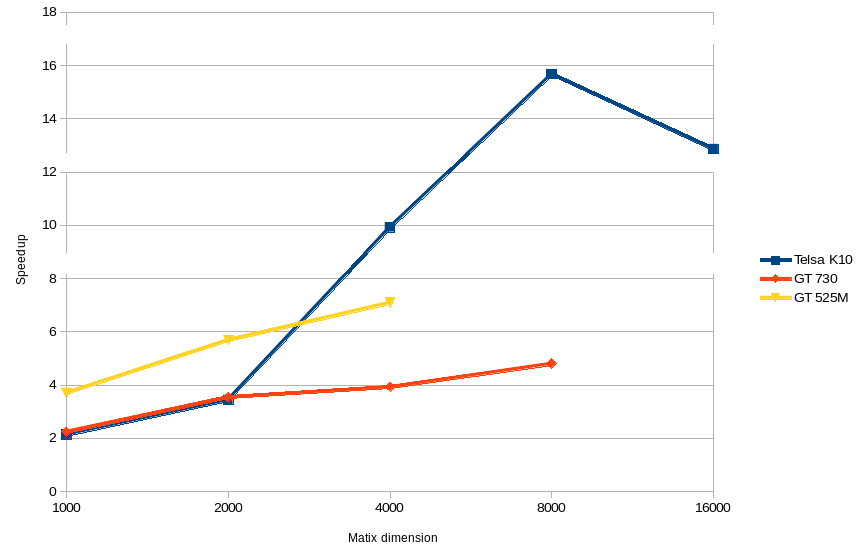
\includegraphics[width=18cm]{figs/speedup.png}
	\centering
	\label{fig:speedup}
	\caption{Speedup of matrix inversion using LU decomposition compared to area-equivalent CPUs}
\end{figure*}

The algorithm based on the Gaussian elimination runs about 60\% faster on CUDA compared to the LU decomposition on big matrices. The difference between the sequential and the CUDA version max out at a speedup of 7 on the Tesla K10 using the Gaussian elimination. The speedup factor of the LU decomposition max out on the same card at a value of around 14. The detailed results are shown in table \ref{tab:results1} and table \ref{tab:results2}.

\begin{table*}
	\begin{tabular}{|c|c|c|c|c|c|c|c|c|c|}\hline
		\rowcolor{black!20} \textbf{Dimension} & \multicolumn{3}{c}{ \textbf{Tesla K10}} & \multicolumn{3}{c}{ \textbf{GT 730}} & \multicolumn{3}{c}{ \textbf{GT 525M}} \\\hline
			\rowcolor{black!20} & CPU & GPU & Speedup & CPU & GPU & Speedup & CPU & GPU & Speedup \\\hline\hline
		1,000 & 1.6 & 0,7 & 2.1 & 5.1 & 2.3 & 2.2 & 7.8 & 2.1 & 3.7 \\\hline
		2,000 & 12.2 & 3,5 & 3.4 & 63 & 17.8 & 3.5 & 88.1 & 15.5 & 5.6 \\\hline
		4,000 & 191.9 & 19,3 & 9.9 & 542 & 138 & 3.9 & 841 & 118 & 7.1 \\\hline
		8,000 & 2462 & 157 & 15.6 & 5368 & 1118 & 4.8 & & & \\\hline
		16,000 & 16250 & 1263 & 12.8 &  & & & & & \\\hline
	\end{tabular}
	\centering
	\label{tab:results1}
	\caption{Detailed execution times of the inversion by LU decomposition algorithm in seconds}
\end{table*}
\begin{table*}
	\begin{tabular}{|c|c|c|c|c|c|c|}\hline
		\rowcolor{black!20} \textbf{Dimension} & \multicolumn{3}{c}{ \textbf{Tesla K10}} & \multicolumn{3}{c}{ \textbf{GT 730}}  \\\hline
		\rowcolor{black!20} & CPU & GPU & Speedup & CPU & GPU & Speedup \\\hline\hline
		1,000 & 1.3 & 1.1 & 1.1 & 0.8 & 1.3 & 0.6 \\\hline
		2,000 & 10.5 & 4.3 & 2.4 & 8.9 & 6.1 & 1.4 \\\hline
		4,000 & 94.3 & 17.2 & 5.4 & 73.5 & 41.9 & 1.7  \\\hline
		8,000 & 660 & 96 & 6.8 & 591 & 337 &  1.7 \\\hline
		16,000 & 5427 & 788  & 6.8  & 4436 & 2694 & 1.6 \\\hline
	\end{tabular}
	\centering
	\label{tab:results2}
	\caption{Detailed execution times of the inversion by Gaussian elimination algorithm in seconds}
\end{table*}

\subsection*{Profiling}
We got another interesting result by running Nvidia's Visual Profiler to compare the computational impact of the single steps of the algorithm.
\vspace{0.2cm}\\
Main computational impact on the sequential algorithm is the inversion step. The inversion takes more than 10 times more time than the LU decomposition.\\
The CUDA version of the algorithm has ratio of about 1:2, i.e. the inversion takes about twice the time as the decomposition. \\ 
The LU decomposition has only a minor speedup on CUDA compared to the CPU. For example the GT 525M is about 1.3 times faster in LU decomposition than the CPU, while the inversion is about 10 times faster (for n=2000).\\
As already mentioned in section (\ref{sec:methods}), the LU decomposition consists of a lot of small grid launched, while the inversion is done by only launching a single grid. 
So one reason for the ''poor'' LU decomposition speedup might be the grid launch overhead. Also an heavy  impact on the speed of the CUDA algorithm is most likely the call of \texttt{cudaMemcpy} in each pivot-finding reduction. In the current version of the algorithm the row-permutation vector is created element by element on the host memory and copied to the GPU memory after the LU decomposition has finished. Even though each call of \texttt{cudaMemcpy} copies only a small amount of data, the CUDA-API calls (\texttt{cudaMemcpy} and grid launch) require a communication of the PCI bus, which has a relatively high latency.
\vspace{0.2cm}\\
So one possible improvement of the LU decomposition algorithm might be to combine some girds and more important to create and keep the row-permutation vector on the GPU memory.
\vspace{0.3cm}\\
The computational impact of each single kernel is shown in figure (\ref{fig:nfprof}). The matrix inversion kernel needs about 64\% of kernel time, the updating of the sub-matrix in the LU decomposition about 35\%. All the other kernels, like row-swap, pivot finding and row-dividing only need less than 1\% of kernel time. 
\begin{figure*}
	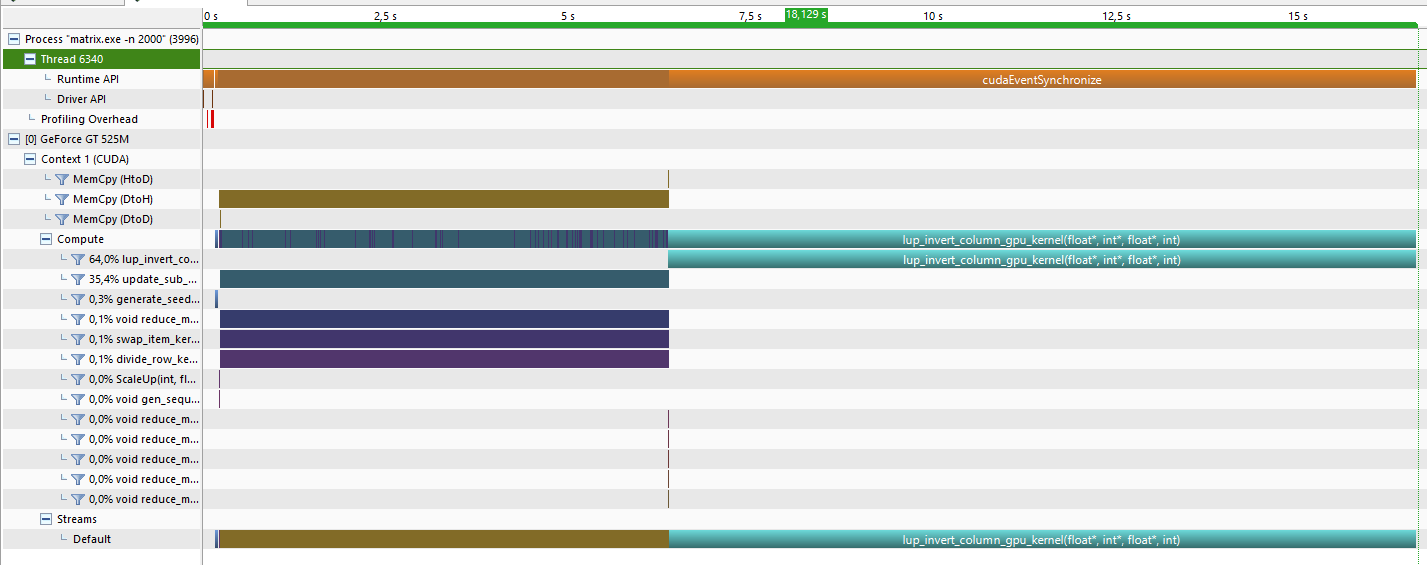
\includegraphics[width=18cm]{figs/nvprof.png}
	\centering
	\label{fig:nfprof}
	\caption{Screenshot of Nvidia's Visual Profiler running the LU decomposition based matrix inversion algorithm}
\end{figure*}

\subsection*{Accuracy}
Due to the limited precision of the used single precision floating point type, the correctness check $A \cdot A^{-1}$ does not always succeed for large dimension $n > 10.000$ and a constant $\varepsilon$. This effect comes out differently on the CPU vs the GPU. The main reason for this behavior is the different instruction sets for allowing the excessive use of \emph{fused-multiply-accumulate} (FMA) instructions on CUDA. As Hokenek et. al \cite{Hokenek90} claims the fusing of arithmetic instructions will increase the accuracy of the computation. In the case of a fused divide and accumulate unit by Amaricai et al. \cite{Amaricai2010} an increase of accuracy up to the factor of 2 can be archived theoretically.
